\chapter{Relevant Theory} \label{ch:ns-equations}
\begin{em}
The methods shown in the previous section describe recursive relationships that build the canonical ensemble. Some of these are numerically unstable while others only apply to a specific spectrum. In an effort to fix these issues, a method that utilizes the grand canonical ensemble will be developed. First, this requires some connection between the canonical and grand canonical ensembles. This connection will be developed in the following section and used to find the occupation probability and extract the temperature. Finally, degenerate spectra will be considered and their error in temperature measurements will be calculated.  
\end{em}
\section{Connecting the Ensembles}
To find a connection between the grand canonical and canonical ensembles, let us return to the partition functions and occupation probabilities discussed in Section 1.2. To begin, consider Equation (1.6) which connects the two ensembles together as 
\begin{equation*}
    Z_{GC}=\sum_{N=0}^{\infty} e^{\beta\mu N} Z_{N}.
\end{equation*}
Using the same idea as Equation (1.9), the probability of being in a single arbitrary state $N$ is 
\begin{equation}
    \avg{p_N}=\frac{e^{\beta\mu N} Z_N}{Z_{GC}}=P(N).
\end{equation}
This equation can be adjusted to read as
\begin{equation}
    Z_N=P(N) Z_{GC} e^{-\beta\mu N}.
\end{equation}
So now there is a connection between the two ensembles. The last two terms make sense in that the difference between the two ensembles is the addition of the chemical potential term. The only term missing is $P(N)$. This is the probability that the grand canonical partition function describes the canonical partition function with $N$ particles. To find this term requires looking more at Equation (2.1).

\section{Poisson Binomial Recursion Relation}
In order to find the probability distribution, $P(N)$, Equation (1.37) needs to be developed further. Rewritten Equation (2.1) using the relationship in Equation (1.12) produces
\begin{equation}
    P(N)=\frac{Z_n e^{\beta\mu N}}{Z_{GC}}=\frac{Z_N e^{\beta\mu N}}{\prod_k \frac{1}{q_k}}= Z_N e^{\beta\mu N} \prod_k q_k.
\end{equation}
From this, a change of variable will be made such that 
\begin{gather}
    \Tilde{Z}_N = B^N Z_N \prod_k A_k\\
    Z_N=\frac{\Tilde{Z}_N}{B^N \prod_k A_k}.
\end{gather}
The values for $B^N$ and $\prod_k A_k$ are $B^N=e^{\beta\mu N}$ and $\prod_k q_k$ from Equation (2.3). They will be used later, but for now Equation (2.5) can be plugged directly into Equation (1.37) to get
\begin{equation}
    Z_N=\frac{\Tilde{Z}_N}{B^N \prod_k A_k} = \frac{\Tilde{Z}_N^{\backslash\{j\}}}{\frac{B^N}{A_j} \prod_k A_k}+e^{-\beta\epsilon_j}\frac{\Tilde{Z}_{N-1}^{\backslash\{j\}}}{\frac{B^{N-1}}{A_j} \prod_k A_k}.
\end{equation}
An important note here is that the division by $A_j$ is to account for the missing energy level $j$. Also, the exponent on the $B$ terms correspond to the number of particles being considered in the original $Z_N^{\backslash\{j\}}$ term. Simplifying this expression gives
\begin{equation}
   \Tilde{Z}_N=A_j \Tilde{Z}_N^{\backslash\{j\}}+ e^{-\beta\epsilon_j} B \Tilde{Z}_{N-1}^{\backslash\{j\}} A_j.
\end{equation}
Now the corresponding values of $A$ and $B$ can be used to produce
\begin{align}
    \Tilde{Z}_N&=q_j \Tilde{Z}_N^{\backslash\{j\}}+ e^{-\beta\epsilon_j} q_j e^{\beta\mu} \Tilde{Z}_{N-1}^{\backslash\{j\}}\nonumber\\
    &=q_j \Tilde{Z}_N^{\backslash\{j\}}+ e^{-\beta(\epsilon_j-\mu)} (1-p_j) \Tilde{Z}_{N-1}^{\backslash\{j\}}\nonumber\\
    &=q_j \Tilde{Z}_N^{\backslash\{j\}}+ e^{-\beta(\epsilon_j-\mu)} \qty(1-\frac{1}{1+e^{\beta(\epsilon_j-\mu)}}) \Tilde{Z}_{N-1}^{\backslash\{j\}}\nonumber\\
    &=q_j \Tilde{Z}_N^{\backslash\{j\}}+ \frac{e^{-\beta(\epsilon_j-\mu)}}{1+e^{-\beta(\epsilon_j-\mu)}} \Tilde{Z}_{N-1}^{\backslash\{j\}}\nonumber\\
    &=q_j \Tilde{Z}_N^{\backslash\{j\}}+ \frac{1}{1+e^{\beta(\epsilon_j-\mu)}} \Tilde{Z}_{N-1}^{\backslash\{j\}}\nonumber\\
    &=q_j \Tilde{Z}_N^{\backslash\{j\}}+ p_j \Tilde{Z}_{N-1}^{\backslash\{j\}}
\end{align}
where $p_j$ is the grand canonical occupation probability and $q_j$ is its compliment. This is a formula to recursively build up $\Tilde{Z}_N$. Next, the definition of $\Tilde{Z}_N$ is found by plugging in the values for $B$ and $A_k$ back into Equation (2.4) to find
\begin{align}
    \Tilde{Z}_N=Z_N B^N \prod_k A_k=Z_N e^{\beta\mu N} \prod_i q_i=\frac{e^{\beta\mu N}Z_N}{Z_{GC}}=P(N).
\end{align}
Plugging this result into (2.8) gives the recursion relationship as
\begin{gather}
    \Tilde{Z}_N=q_j \Tilde{Z}_N^{\backslash\{j\}}+ p_j \Tilde{Z}_{N-1}^{\backslash\{j\}}\\
    P_N=q_j P_N^{\backslash\{j\}}+ p_j P_{N-1}^{\backslash\{j\}}\\
    P_j(N)=q_j P_j(N)+p_j P_{j-1}(N-1)
\end{gather}
where the final step is performed to simplify notation for later. This is the missing probability distribution needed in Equation (2.2). Moreover, there is now a recursive method to find the probability that the grand canonical partition function accurately represents a canonical partition function of $N$ particles. This recursion has many interesting properties. To start, it adds on a value to the distribution each iteration. When at position $N+1$, the $p_j P_{N-1}^{\backslash\{j\}}$ term still contributes a nonzero value to the probability. This means that iterating over all possible $j$ values for $p$ and $q$ will give a distribution that is $N$ values long. This can be viewed in the form of a triangle where the base is constantly extended with each iteration. This creates a sort of pascal triangle. To build some intuition of this, let us consider another short example. To start, let the probability distribution and it's compliment be
\begin{gather}
    p=\qty[1,\frac{1}{2},\frac{1}{3},\frac{1}{6}]\nonumber\\
    q=1-p=\qty[1,\frac{1}{2},\frac{2}{3},\frac{5}{6}]\nonumber.
\end{gather}
where each term in the array corresponds to the probability that a particle occupies (or doesn't occupy) that state. By summing the values in the probability distribution, the total number of particles is expected to be 2. From here, the recursive relationship can be initialized with a value of $P_0(1)=0$. The calculation can then continue until all values in the probability distribution are used. This is done to show
\begin{gather*}
    P_1(1)=p_1 P_{0}(0)+q_1 P_{0}(1)=(1)(0)+(0)(1)=0\\
    P_1(2)=p_1 P_{0}(1)+q_1 P_{0}(2)=(1)(1)+(0)(0)=1\\
    P_1=[0,1]\\
    P_2(1)=p_2 P_{1}(0)+q_2 P_{1}(1)=\qty(\frac{1}{2})(0)+\qty(\frac{1}{2})(0)=0\\
    P_2(2)=p_2 P_{1}(1)+q_2 P_{1}(2)=\qty(\frac{1}{2})(0)+\qty(\frac{1}{2})(1)=\frac{1}{2}\\
    P_2(3)=p_2 P_{1}(2)+q_2 P_{1}(3)=\qty(\frac{1}{2})(1)+\qty(\frac{1}{2})(0)=\frac{1}{2}\\
    P_2=\qty[0,\frac{1}{2},\frac{1}{2}]\\
    P_3(1)=p_3 P_{2}(0)+q_3 P_{2}(1)=\qty(\frac{2}{3})(0)+\qty(\frac{1}{3})(0)=0\\
    P_3(2)=p_3 P_{2}(1)+q_3 P_{2}(2)=\qty(\frac{2}{3})\qty(\frac{1}{2})+\qty(\frac{1}{3})(0)=\frac{1}{3}\\
    P_3(3)=p_3 P_{2}(2)+q_3 P_{2}(3)=\qty(\frac{2}{3})\qty(\frac{1}{2})+\qty(\frac{1}{3})\qty(\frac{1}{2})=\frac{1}{2}\\
    P_3(4)=p_3 P_{2}(4)+q_3 P_{2}(4)=\qty(\frac{2}{3})(0)+\qty(\frac{1}{3})\qty(\frac{1}{2})=\frac{1}{6}\\
    P_3=\qty[0,\frac{1}{3},\frac{1}{2},\frac{1}{6}]\\
    P_4(1)=p_4 P_{3}(0)+q_4 P_{3}(1)=\qty(\frac{5}{6})(0)+\qty(\frac{1}{6})(0)=0\\
    P_4(2)=p_4 P_{3}(1)+q_4 P_{3}(2)=\qty(\frac{5}{6})\qty(\frac{1}{3})+\qty(\frac{1}{6})(0)=\frac{10}{36}\\
    P_4(3)=p_4 P_{3}(2)+q_4 P_{3}(3)=\qty(\frac{5}{6})\qty(\frac{1}{2})+\qty(\frac{1}{6})\qty(\frac{1}{3})=\frac{17}{36}\\
    P_4(4)=p_4 P_{3}(4)+q_4 P_{3}(4)=\qty(\frac{5}{6})\qty(\frac{1}{6})+\qty(\frac{1}{6})\qty(\frac{1}{2})=\frac{8}{36}\\
    P_4(5)=p_4 P_{3}(4)+q_4 P_{3}(4)=\qty(\frac{5}{6})(0)+\qty(\frac{1}{6})\qty(\frac{1}{6})=\frac{1}{36}\\
    P_4=\qty[0,\frac{10}{36},\frac{17}{36},\frac{8}{36},\frac{1}{36}].
\end{gather*}
This solution can be visualized as a triangle as seen in Fig.(2.1). 
\begin{figure}[H]
    \centering
    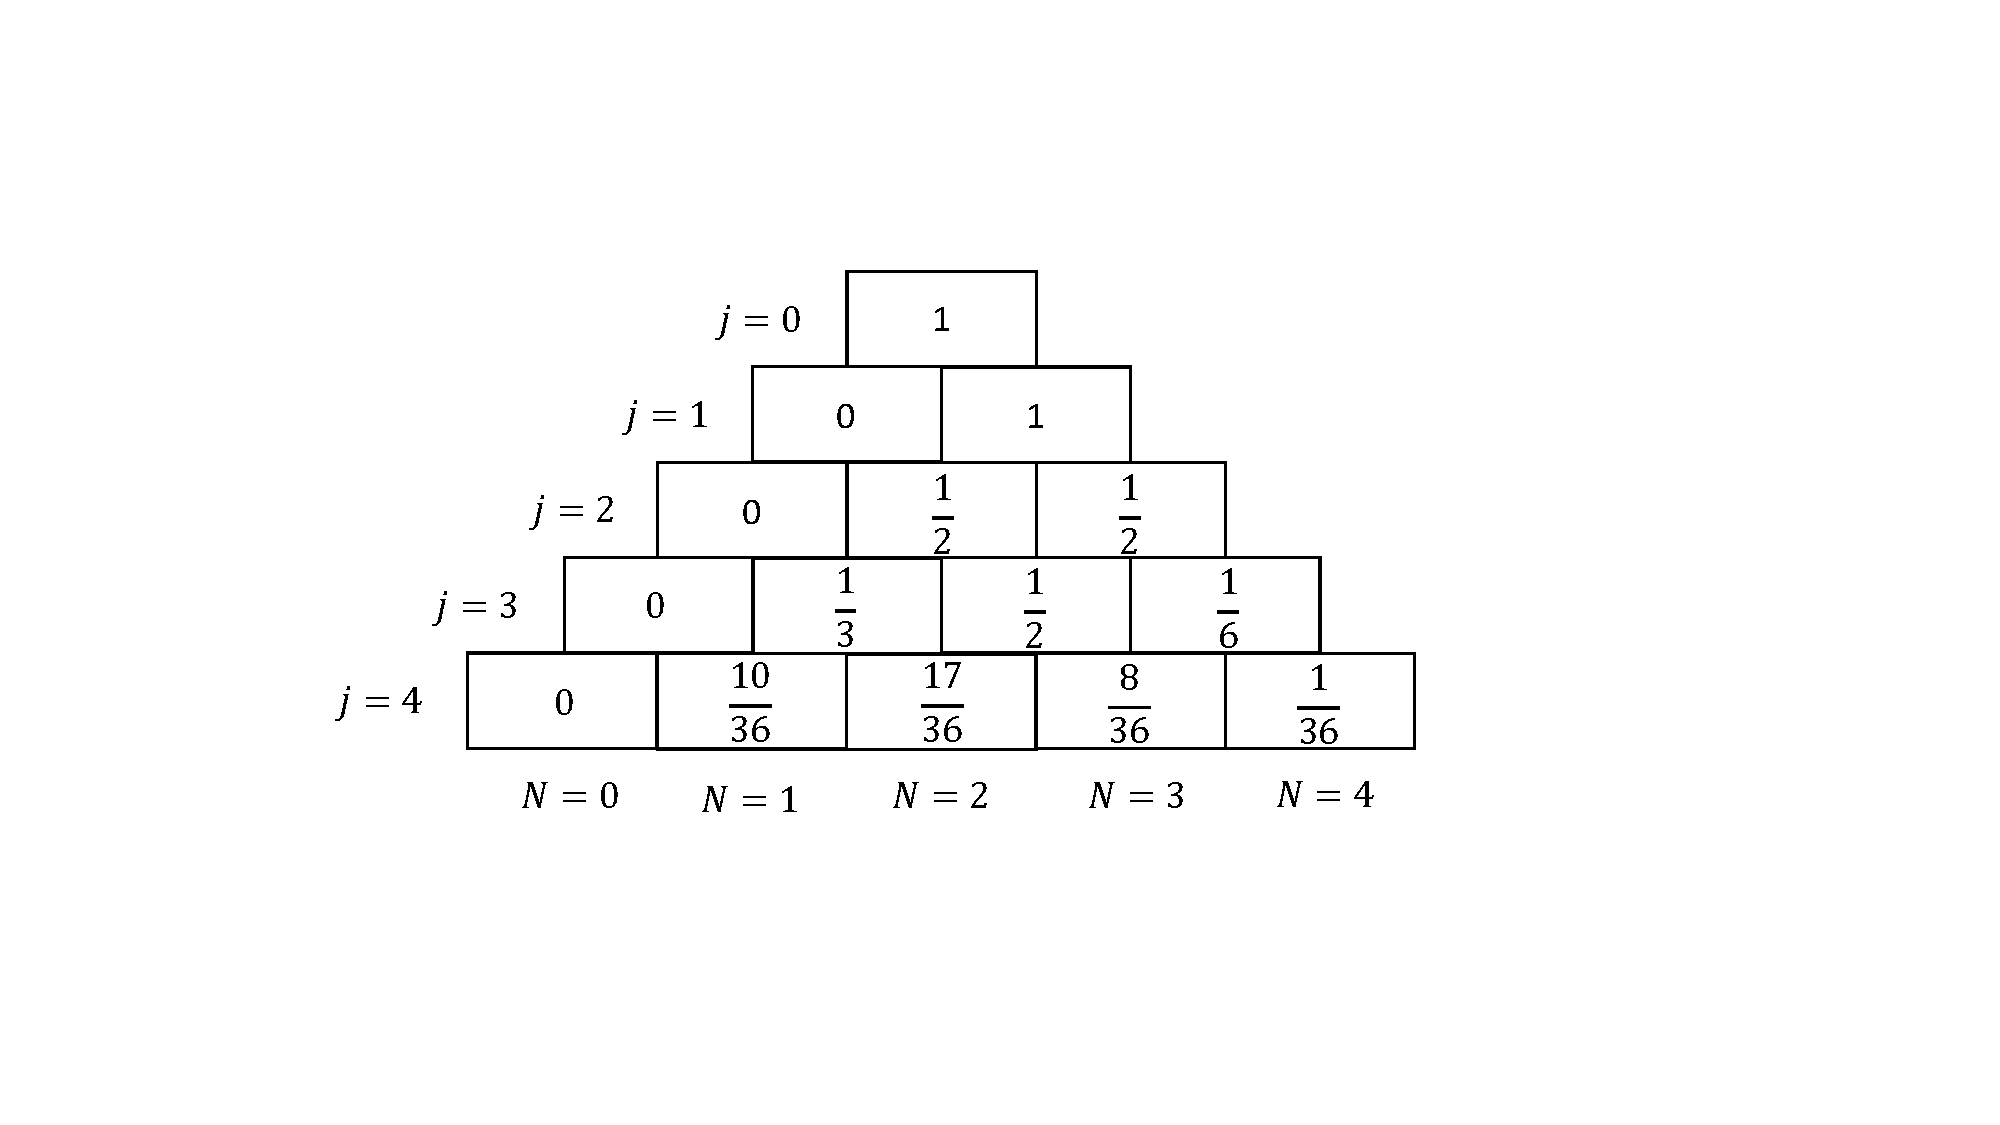
\includegraphics[scale=0.55]{figures/pdf/PBTriangle.pdf}
    \caption{Poisson Binomial Triangle.}
    \label{fig:Poisson Binomial Triangle}
\end{figure}
A more general visualization of this triangle can be seen in Fig.(2.2)
\begin{figure}[H]
    \centering
    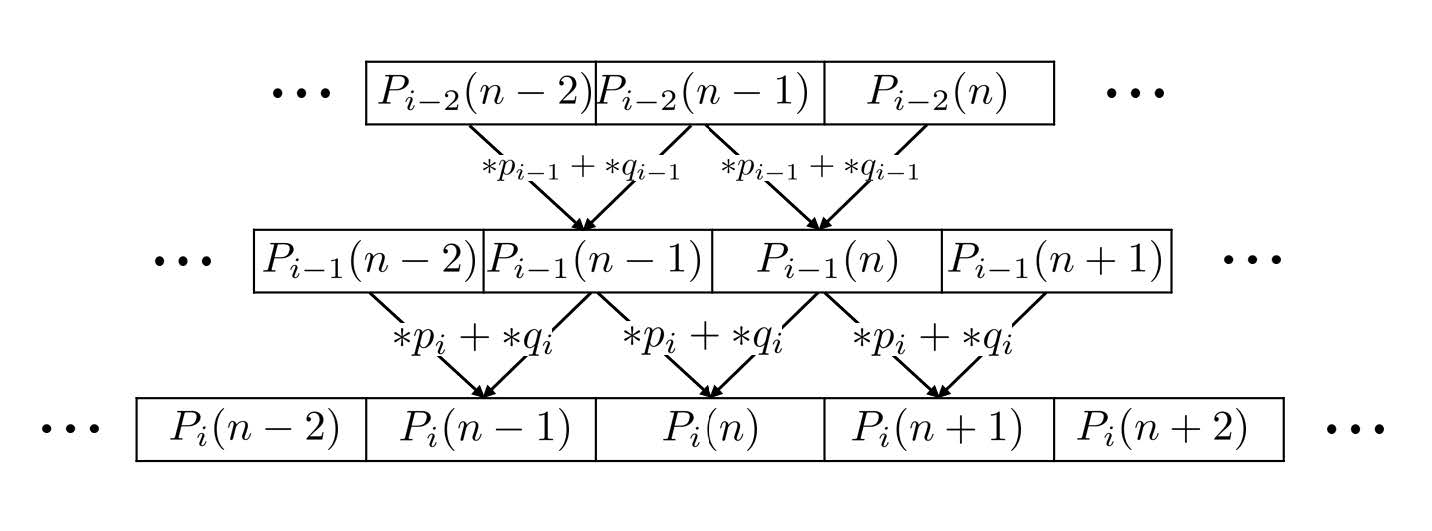
\includegraphics[scale=0.8]{figures/pdf/PBrecursion.jpg}
    \caption{General Poisson Binomial Recursion}
    \label{fig:General Poisson Binomial Recursion}
\end{figure}
As expected, the highest probability corresponds to having $N=2$ particles. Another nice feature of this method is that the probability is normalized. Equation (1.37) has no normalization condition or any reason to be normalized given that the canonical partition function's only restriction is on the number of particles.


\section{Occupation Probability from recursion}
The occupation probability for the canonical ensemble can now be calculated from the Equation (2.12). Rewriting this equation gives
\begin{equation}
    1=\frac{q_j P_{j-1}(N)}{P_j(N)} + \frac{p_j P_{j-1}(N-1)}{P_j(N)}.
\end{equation}
Inspecting this equation, the right fraction is the probability of occupying energy level $j$ and $N-1$ other energy levels. The left fraction is the probability of not occupying energy level $j$ and $N$ other energy levels. This explanation follows from the same idea as the two parts of Equation (1.37). Therefore, the occupation probability for the canonical ensemble is the right fraction on the right hand side of Equation (2.13). Specifically,
\begin{equation}
    \avg{n}_j=\frac{p_j P_{j-1}(N-1)}{P_j(N)}.
\end{equation}

\section{Temperature Extraction}
The occupation probability can now be used to find the correct temperature of the system. To do this, the value of $\beta$ in the original probability distribution is varied until it matches the calculated canonical occupation probability. To do this, the function 
\begin{equation}
    \chi^2=\sum_j(p_j-n_j)^2
\end{equation}
is implemented. The choice of the occupation probability $p$ is of the form of Equation (1.16). The $\mu$ term is set so that the sum of all probabilities equals the number of particles in the system. Therefore, the only term that can be tuned is the temperature dependence of $p_j$, which is $\beta^*$. Since it is dependent only on $\beta^*$, the first and second derivatives can be calculated and used to find the minimum. This is fully calculated in Appendix B, but the important results are 
\begin{gather}
    \frac{d\chi^2}{d\beta^*}=\sum_j -2(p_j-n_j)p_j q_j \epsilon_j+\sum_j 2(p_j-n_j)p_j q_j C_1\\
    \frac{d^2\chi^2}{d\beta^{*2}}=2\sum_j\Biggr[(\epsilon_j-C_1)^2[(p_j-n_j)p_jq_j(q_j-p_j)+p_j^2q_j^2]\nonumber\\
    \ \ \ \ \ \ +(p_j-n_j)p_jq_j(C_1C_3+C_2)\Biggr]\\
    C_1=\frac{\sum_j \epsilon_j p_j q_j}{\sum_j p_j q_j}\\
    C_2=\frac{\sum_j \epsilon_j p_j q_j(p_j - q_j)(\epsilon_j-C_1)}{\sum_j p_j q_j}\\
    C_3=\frac{\partial C_1}{\partial y}=\frac{\partial}{\partial 
    y}\qty{\frac{\sum_j \epsilon_j q_j p_j}{\sum_j p_j q_j}}=\frac{\sum_j p_j q_j(q_j-p_j)(\epsilon_j-C_1)}{\sum_j p_j q_j}.
\end{gather}
With both derivatives available, Newton's method of optimization can be used to find the correct value of $\beta^*$. This method involves using 
\begin{equation}
    \beta^*=\beta^*-\frac{\partial_{\beta^*}\chi^2}{\partial^2_{\beta^*}\chi^2}
\end{equation}
to iterate through the $\chi^2$ function until the minimum is found.

\section{Degenerate energy spectra}
Now the case of degenerate energy spectra will be considered. To begin, define the degeneracy of a certain energy level $i$ as $g_i$. The canonical partition function is written as
\begin{equation}
    Z_k(\epsilon_i;g_i)={g_i \choose k} e^{-k\beta\epsilon_i}
\end{equation}
with $k$ being the number of particles at level $i$.  For the purpose of this calculation, $\beta$ is sufficiently large so that the only excitations will be around Fermi energy level. In this scenario, there are two cases of interest. These are when the degenerate Fermi level is filled and partially filled. 
\subsection{Filled Degenerate Fermi Level}
The first case to consider is when the Fermi level is degenerate and filled. In this case, there are only two levels to worry about, the Fermi level and the first excited state. All other levels are filled or empty. To begin, let $i=0$ denote the Fermi level and $i=1$ denote the first excited state. Since these two levels are the only ones of interest, the simple example in Section 1.3 can be revisited. Consider there is one particle in a system where the Fermi level has degeneracy $g_0$ and energy $\epsilon_0$ and the first excited state has degeneracy $g_1$ and energy $\epsilon_1$. For convenience, the energy spectrum can be redefined as
\begin{equation}
    \epsilon_0 \xrightarrow[]{} 0\ \ \ \ \ \epsilon_1\xrightarrow[]{}\Delta_0=\epsilon_1-\epsilon_1.\nonumber
\end{equation}
The partition function for this case can be written from (1.32) to yield
\begin{align}
    Z_{g_0}(0,\Delta_0;g_0,g_1)&=\sum_{k=0}^{\text{min}(g_1,g_0)} Z_k(\Delta_0,g_1)Z_{g_0-k}(0,g_0)\nonumber\\
    &=\sum_{k=0}^{\text{min}(g_1,g_0)} {g_1 \choose k}{g_0\choose g_0-k} e^{-\beta \epsilon_0 k}e^{-\beta \epsilon_1 k}\nonumber\\
    &=\sum_{k=0}^{\text{min}(g_1,g_0)} {g_1 \choose k}{g_0\choose g_0-k} e^{-\beta \Delta_0 k}
\end{align}
where the $\text{min}(g_1,g_0)$ represents the minimum of the two values. The minimum is used here because there can only be as many particles as there are available positions in the energy level. For non degenerate case, this would be one, but for the degenerate case, this can be an arbitrary positive integer value. The canonical occupation probability can be calculated the same as before by leaving out an energy level and multiplying by its Boltzmann factor. This results in 
\begin{align}
    \avg{n_0}_{g_0}&=\frac{e^{-\beta \epsilon_0}Z_{g_0-1}(0,\Delta_0;g_0-1,g_1)}{Z_{g_0}(0,\Delta_0;g_0,g_1)}\nonumber\\
    &=\frac{\sum_{k=0}^{\text{min}(g_1,g_0-1)} {g_1 \choose k}{g_0\choose g_0-1-k} e^{-\beta \Delta_0 k}}{\sum_{k=0}^{\text{min}(g_1,g_0)} {g_1 \choose k}{g_0\choose g_0-k} e^{-\beta \Delta_0 k }}\nonumber\\
    &=\frac{{g_1\choose 0}{g_0-1\choose g_0-1}+{g_1 \choose 1}{g_0-1\choose g_0-2}e^{-\beta\Delta_0}+{g_1\choose 2}{g_0-1\choose g_0-3}e^{-2\beta\Delta_0}+...}{{g_1\choose 0}{g_0\choose g_0}+{g_1 \choose 1}{g_0\choose g_0-1}e^{-\beta\Delta_0}+{g_1\choose 2}{g_0-1\choose g_0-2}e^{-2\beta\Delta_0}+...}\nonumber\\
    &=\frac{1+g_1(g_0-1)e^{-\beta\Delta_0}+\frac{g_1(g_1-1)(g_0-1)(g_0-2)}{4}e^{-2\beta\Delta_0}+...}{1+g_0g_1e^{-\beta\Delta_0}+\frac{g_1(g_1-1)g_0(g_0-1)}{4}e^{-2\beta\Delta_0}+...}.
\end{align}
Similarly, for the first excited state,
\begin{align}
    \avg{n_1}_{g_0}&=\frac{e^{-k\epsilon_1} Z_{g_0-1}(0,\Delta_0;g_0,g_1-1)}{Z_{g_0}(0,\Delta_0;g_0,g_1)}\nonumber\\
    &=\frac{e^{-k\Delta_0}\sum_{k=0}^{\text{min}(g_1-1,g_0-1)} {g_1-1\choose k}{g_0 \choose k+1} e^{-k\beta\Delta_0}}{\sum_{k=0}^{\text{min}(g_1,g_0)} {g_1\choose k}{g_0 \choose k} e^{-k\beta\Delta_0}}\nonumber\\
    &=\frac{{g_1-1\choose 0}{g_0\choose 1} e^{-\beta\Delta_0} +{g_1-1\choose 1}{g_0\choose 2} e^{-2\beta\Delta_0}+{g_1-1\choose 2}{g_0\choose 3}e^{-3\beta\Delta_0}+...}{{g_0\choose 0}{g_1\choose 0}+{g_0\choose 1}{g_1\choose 1}e^{-\beta\Delta_0}+{g_0\choose 2}{g_1\choose 2}e^{-2\beta\Delta_0}+...}\nonumber\\
    &=\frac{g_0e^{-\beta\Delta_0}+\frac{(g_1-1)g_0(g_0-1)}{2}e^{-2\beta\Delta_0}+...}{1+g_0g_1 e^{-\beta\Delta_0}+\frac{g_1(g_1-1)g_0(g_0-1)}{4}e^{-2\beta\Delta_0}+...}.
\end{align} 
Like before, the chemical potential can be found by using the grand canonical probabilities $p_0$ and $p_1$ such that,
\begin{gather}
    p_0=\frac{1}{1+e^{\beta^*(\epsilon_0-\mu)}}=\frac{1}{1+e^{-\beta^* \mu}}\\
    p_1=\frac{1}{1+e^{\beta^*(\epsilon_0-\mu)}}=\frac{1}{1+e^{\beta^*(\Delta_0-\mu)}}\\
    p_0g_0+p_1g_1=g_0.
\end{gather}
Plugging everything in gives
\begin{gather}
    g_0=\frac{g_0}{1+e^{\beta^*(\epsilon_0-\mu)}}=\frac{1}{1+e^{-\beta^*\mu}}+\frac{g_1}{1+e^{\beta^*(\epsilon_0-\mu)}}=\frac{1}{1+e^{\beta^*(\Delta_0-\mu)}}\nonumber\\
    1+e^{\beta^*\Delta_0} e^{-\beta^*\mu}+\frac{g_1}{g_0}(1+e^{-\beta^*\mu})=(1+e^{-\beta^*\mu})(1+e^{\beta^*\Delta_0} e^{-\beta^* \mu})\nonumber\\
    1+e^{-\beta^*\mu}(\frac{g_1}{g_0}+e^{\beta^*\Delta_0})+\frac{g_1}{g_0}=1+e^{-\beta^*\mu}+e^{\beta^*\Delta_0}e^{-\beta^*\mu}+e^{-2\beta^*\mu}e^{\beta^*\Delta_0}\nonumber\\
    0=(e^{-\beta^*\mu})^2 e^{\beta^*\Delta_0} +e ^{-\beta^*\mu}(1-\frac{g_1}{g_0})-\frac{g_1}{g_0}.
\end{gather}
This is a simple quadratic equation so there will be two solutions. To have a real solution, the positive root is kept resulting in
\begin{align}
    e^{-\beta^*\mu}&=\frac{(\frac{g_1}{g_0}-1)\pm\sqrt{(\frac{g_1}{g_0}-1)^2+4e^{\beta^*\Delta_0}\frac{g_1}{g_0}}}{2e^{\beta^*\Delta_0}}\nonumber\\
    &=\frac{e^{-\beta^*\Delta_0}}{2}(\frac{g_1}{g_0}-1)\pm \frac{1}{2}\sqrt{e^{-2\beta^*\Delta_0} (\frac{g_1}{g_0}-1)^2+ 4e^{-\beta^*\Delta_0}\frac{g_1}{g_0}}.
\end{align}
Just like the simple example before, set the canonical and grand canonical probabilities to be equal, such that $\avg{n_0}_{g_0}=p_0$. This gives 
\begin{align}
    \frac{1}{\avg{n_0}_{g_0}}-1=\frac{1}{p_0}-1=1+e^{-\beta^*\mu}-1=e^{-\beta^*\mu} .
\end{align}
Now there is a connection to the grand canonical probability to the canonical probability for the degenerate case. Setting the two $e^{-\beta^*\mu}$ terms equal to one another yields
\begin{gather}
    \frac{1}{\avg{n_0}_{g_0}}-1=\frac{e^{-\beta^*\Delta_0}}{2}(\frac{g_1}{g_0}-1)\pm \frac{1}{2}\sqrt{e^{-2\beta^*\Delta_0} (\frac{g_1}{g_0}-1)^2+ 4e^{-\beta^*\Delta_0}\frac{g_1}{g_0}}\nonumber\\
    2\frac{1-\avg{n_0}_{g_0}}{\avg{n_0}_{g_0}}-e^{-\beta^*\Delta_0}(\frac{g_1}{g_0}-1)=\sqrt{e^{-2\beta^*\Delta_0} (\frac{g_1}{g_0}-1)^2+ 4e^{-\beta^*\Delta_0}\frac{g_1}{g_0}}\nonumber\\
    4\qty(\frac{1-\avg{n_0}_{g_0}}{\avg{n_0}_{g_0}})^2-4e^{-\beta^*\Delta_0}\qty(\frac{g_1}{g_0}-1) \frac{1-\avg{n_0}_{g_0}}{\avg{n_0}_{g_0}}+e^{-2\beta^*\Delta_0} \qty(\frac{g_1}{g_0}-1)^2\nonumber\\ 
    \ \ \ \ \ \ \  =e^{-2\beta^*\Delta_0} (\frac{g_1}{g_0}-1)^2+ 4e^{-\beta^*\Delta_0}\frac{g_1}{g_0} \nonumber\nonumber\\
    0=4\qty(\frac{1-\avg{n_0}_{g_0}}{\avg{n_0}_{g_0}})^2- 4e^{-\beta^*\Delta_0}\qty(\qty(\frac{g_1}{g_0}-1)\frac{1-\avg{n_0}_{g_0}}{\avg{n_0}_{g_0}}+\frac{g_1}{g_0})\nonumber\\
    4\qty(\frac{1-\avg{n_0}_{g_0}}{\avg{n_0}_{g_0}})^2=4e^{-\beta^*\Delta_0}\qty(\qty(\frac{g_1}{g_0}-1)\frac{1-\avg{n_0}_{g_0}}{\avg{n_0}_{g_0}}+\frac{g_1}{g_0})\nonumber\\
    e^{\beta^* \Delta_0}=\frac{1-\avg{n_0}_{g_0}}{\avg{n_0}_{g_0}}(\frac{g_1}{g_0}-1)+\qty(\frac{1-\avg{n_0}_{g_0}}{\avg{n_0}_{g_0}})^2\frac{g_1}{g_0}.
\end{gather}
With this definition, $\frac{1-\avg{n_0}_{g_0}}{\avg{n_0}_{g_0}}$ terms are worked out and plugged in. This is done in Appendix C.1. An important note for these calculations is that terms greater than $\mathcal{O}\qty(e^{-2\beta \Delta_0})$ are neglected because they will be sufficiently small. Using Equations (C.8) and (C.9),
\begin{align}
    e^{\beta^* \Delta_0}&=\frac{e^{\beta\Delta_0}}{g_1}\qty(1+\frac{(g_1+1)(g_0-1)}{2}e^{-\beta\Delta_0})\qty(\frac{g_1}{g_0}-1)\nonumber\\
    &\ \ \ \ \ \ \ \ \ \ +\frac{e^{2\beta\Delta_0}}{g_1^2}\qty(1+(g_1+1)(g_0-1)e^{-\beta\Delta_0})\frac{g_1}{g_0}\nonumber\\
    &=\frac{e^{2\beta\Delta_0}}{g_1g_0}\qty((g_1-g_0)e^{-\beta\Delta_0}+f+(g_1+1)(g_0-1)e^{-\beta\Delta_0})\nonumber\\
    &=\frac{e^{2\beta\Delta_0}}{g_1g_0}\qty((g_1g_0-1)e^{-\beta\Delta_0}+1)\\
    \beta^*\Delta_0&=2\beta\Delta_0-\ln(g_0g_1)+\ln\qty((g_1g_0-1)e^{-\beta\Delta_0}+1).
\end{align}
Since $e^{-\beta\Delta_0}$ is small, the third term on the right hand size can be approximated using $\ln(1+x)\approx x$. This yields
\begin{align}
    \beta^*\Delta_0&=2\beta\Delta_0-\ln\qty(g_0g_1)+(g_1g_0-1)e^{-\beta\Delta_0}\nonumber\\
    \beta^*&=2\beta-\frac{\ln\qty(g_0g_1)}{\Delta_0}+\frac{g_1g_0-1}{\Delta_0}e^{-\beta\Delta_0}.
\end{align} 
This is the relationship between the canonical temperature and the grand canonical temperature. This can be rewritten in terms of the error of the grand canonical $\beta^*$ value. For this, consider 
\begin{align}
    \frac{\beta^*-\beta}{\beta}=\frac{\delta\beta}{\beta}=1-\frac{\ln(g_0g_1)}{\beta\Delta_0}+\frac{(g_1g_0 - 1)}{\beta \Delta_0}e^{-\beta\Delta_0}.
\end{align}
To check if this is accurate, this equation should give the same results when the degeneracies are removed.
\begin{gather}
    g_0=g_1=1\nonumber\\
    \frac{\delta\beta}{\beta}=1-\frac{\ln(1)}{C_1}+\frac{(1)(1)-1}{C_2}=1\nonumber
\end{gather}
This is the condition for the nondegenerate case, so the filled degenerate fermi level theory matches the nondegenerate theory. 
\subsection{Partially Filled Degenerate Fermi Level}
Turning to the case of a partially filled degenerate energy spectrum, consider that the Fermi level is partially filled. This setup requires considering both the level above and below the Fermi level. The energy spectrum can be rewritten as 
\begin{gather}
    \epsilon_0 \xrightarrow[]{} 0\nonumber\\
    \epsilon_1 \xrightarrow[]{} \Delta_0=\epsilon_1-\epsilon_0\nonumber\\
    \epsilon_{-1} \xrightarrow[]{} -\Delta_{-1}=\epsilon_{-1}-\epsilon_0.\nonumber
\end{gather}
The number of particles in the partially filled level will be denoted as $\ell$. The partition function for this case is 
\begin{align}
    &Z_{g_{-1}+\ell}(-\Delta_{-1},0,\Delta;g_{-1},g_0,g_1) = e^{g_{-1}\beta\Delta_{-1}} \Biggr[{g_0\choose \ell}+g_1{g_0\choose \ell-1}e^{-\beta\Delta_0} \nonumber\\
    &\quad +g_{-1}{g_0\choose \ell+1}e^{-\beta\Delta_{-1}} +\frac{g_1(g_1-1)}{2} {g_0\choose \ell-2}e^{-2\beta\Delta_0}\nonumber\\ 
    &\quad +\frac{g_{-1}(g_{-1}-1)}{2} {g_0\choose \ell+2} e^{-2\beta\Delta_{-1}} +g_1g_{-1}{g_0\choose \ell} e^{-\beta(\Delta_0+\Delta_{-1})} \Biggr]\nonumber\\
    &\ \ =e^{g_{-1}\beta\Delta_{-1}} {g_0\choose \ell} \Biggr[1+ \frac{g_1 \ell}{g_0-\ell+1} e^{-\beta\Delta_0} +\frac{g_{-1}(g_0-\ell)}{\ell+1} e^{-\beta\Delta_{-1}} \nonumber\\
    &\quad+\frac{g_1(g_1-1)}{2} \frac{\ell(\ell-1)}{(g_0+\ell+1)(g_0+\ell+2)}e^{-2\beta\Delta_0} \nonumber\\
    &\quad+\frac{g_{-1}(g_{-1}-1)}{2} \frac{(g_0-\ell)(g_0-\ell-1)}{(\ell+1)(\ell+2)} e^{-2\beta\Delta_{-1}}+g_1g_{-1}e^{-\beta(\Delta_0+\Delta_{-1})}\Biggr].
\end{align}
As before, the partition function can be found for states with one particle removed. For level $i=-1$,
\begin{align}
    &Z_{g_{-1}+\ell-1}(-\Delta_{-1},0,\Delta_0;g_{-1}-1,g_0,g_1)=e^{(g_{-1}-1)\beta\Delta_{-1}} {g_0\choose \ell} \Biggr[1+\frac{g_1 \ell}{g_0-\ell+1} e^{-\beta\Delta_0} \nonumber\\
    &\quad +\frac{(g_{-1}-1)(g_0-\ell)}{\ell+1} e^{-\beta\Delta_{-1}}+\frac{g_1(g_1-1)}{2} \frac{\ell(\ell-1)}{(g_0+\ell+1)(g_0+\ell+2)}e^{-2\beta\Delta_0} \nonumber\\
    &\quad+\frac{(g_{-1}-1)(g_{-1}-2)}{2} \frac{(g_0-\ell)(g_0-\ell-1)}{(\ell+1)(\ell+2)} e^{-2\beta\Delta_{-1}}+g_1(g_{-1}-1)e^{-\beta(\Delta_0+\Delta_{-1})}\Biggr].
\end{align}
For level $i=0$,
\begin{align}
    &Z_{g_{-1}+\ell-1}(-\Delta_{-1},0,\Delta_0;g_{-1},g_0-1,g_1)=e^{g_{-1}\beta\Delta_{-1}} {g_0-1\choose \ell-1} \Biggr[1+\frac{g_1 (\ell-1)}{g_0-\ell-1} e^{-\beta\Delta_0}\nonumber\\
    &\quad+\frac{g_{-1}(g_0-\ell)}{\ell} e^{-\beta\Delta_{-1}} +\frac{g_1(g_1-1)}{2} \frac{(\ell-1)(\ell-2)}{(g_0+\ell+1)(g_0+\ell+2)}e^{-2\beta\Delta_0}\nonumber\\ &\quad+\frac{g_{-1}(g_{-1}-1)}{2} \frac{(g_0-\ell)(g_0-\ell-1)}{\ell(\ell+1)} e^{-2\beta\Delta_{-1}} +g_1g_{-1}e^{-\beta(\Delta_0+\Delta_{-1})}\Biggr].
\end{align}
For level $i=1$,
\begin{align}
    &Z_{g_{-1}+\ell}(-\Delta_{-1},0,\Delta;g_{-1},g_0,g_1-1) =e^{g_{-1}\beta\Delta_{-1}} {g_0\choose \ell-1} \Biggr[1+\frac{(g_1-1) (\ell-1)}{g_0-\ell-1} e^{-\beta\Delta_0} \nonumber\\
    &\quad+\frac{g_{-1}(g_0-\ell+1)}{\ell} e^{-\beta\Delta_{-1}} +\frac{(g_1-1)(g_1-2)}{2} \frac{(\ell-2)(\ell-3)}{(g_0+\ell+2)(g_0+\ell+3)}e^{-2\beta\Delta_0}\nonumber\\ &\quad+\frac{g_{-1}(g_{-1}-1)}{2} \frac{(g_0-\ell+1)(g_0-\ell)}{(\ell-1)\ell} e^{-2\beta\Delta_{-1}} +g_1g_{-1}e^{-\beta(\Delta_0+\Delta_{-1})}\Biggr].
\end{align}
As before, the grand canonical occupation probability are written as,
\begin{gather}
    p_1=\frac{1}{1+e^{\beta^*(\Delta_1-\mu)}}\nonumber\\
    p_0=\frac{1}{1+e^{-\beta^*\mu}}\nonumber\\
    p_{-1}=\frac{1}{1+e^{\beta^*(\Delta_{-1}-\mu)}}\nonumber
\end{gather}
The chemical potential is found from the particle number. This is worked out in Appendix C.2, but the solution is shown below. 
\begin{align}
    &0=e^{-3\beta^*\mu}(e^{\beta^*(\Delta_1+\Delta_{-1})})\nonumber\\
    &+e^{-2\beta^*\mu}\Biggr(e^{\beta^*\Delta_1}+e^{\beta^*\Delta_{-1}}+e^{\beta^*(\Delta_{-1}+\Delta_1)}-\frac{g_1}{g_{-1}+\ell}e^{\beta^*\Delta_{-1}}\nonumber-\frac{g_0}{g_{-1}+\ell}e^{\beta^*(\Delta_1+\Delta_{-1})}\nonumber\\
    &\quad\quad\quad\quad\ \ \ -\frac{g_{-1}}{g_{-1}+\ell}e^{\beta^*\Delta_1}\Biggr)\nonumber\\
    &+e^{-\beta^*\mu}\Biggr(1+e^{\beta^*\Delta_1}+e^{\beta^*\Delta_{-1}}-\frac{g_1}{g_{-1}+\ell}(1+e^{\beta^*\Delta_{-1}})-\frac{g_0}{g_{-1}+\ell}(e^{\beta^*\Delta_1}+e^{\beta^*\Delta_{-1}})\nonumber\\
    &\quad\quad\quad\quad\ \ -\frac{g_{-1}}{g_{-1}+\ell}(1+e^{\beta^*\Delta_1})\Biggr)\nonumber\\
    & +(1-\frac{g_1}{g_{-1}+\ell}-\frac{g_0}{g_{-1}+\ell}-\frac{g_{-1}}{g_{-1}+\ell})
\end{align}
This is a cubic equation with roots that contain $e^{-\beta^*\Delta_0}$ and $e^{-\beta^*\Delta_{-1}}$. 
Given this equation, there are more variables than equations describing this case, so an exact solution cannot be found. Therefore, it's desirable to turn this into a two level system. To do so, consider that either $\Delta_0$ or $\Delta_{-1}$ is large enough that any excitations to or from that level are negligible. These two cases are discussed in the following sections. 

\subsubsection{Case 1: $\beta^*(\Delta_{-1}-\Delta_0)\gg 1$}
For this case, the gap between the excited state and the Fermi level is much smaller than the gap between the state below and the Fermi level. For this case, the excitations from the $i=-1$ level can be ignored. This brings the problem back to a two level system that can be exactly solved. The occupation probability is then defined as
\begin{align}
    \avg{n_0}_\ell&=\frac{Z_{\ell-1}(0,\Delta_0;g_0-1,g_1)}{Z_\ell(0,\Delta_0;g_0,g_1)}\nonumber\\
    &=\frac{{g_0-1\choose \ell-1}[1+\frac{g_1(\ell-1)}{g_0-\ell+1}e^{-\beta\Delta_0} +\frac{g_1(g_1-1)(\ell-1)(\ell-2)}{2(g_0-\ell+1)(g_0-\ell+2)}e^{-2\beta\Delta_0}]}{{g_0\choose \ell}[1+\frac{g_1 \ell}{g_0-\ell+1}e^{-\beta\Delta_0} +\frac{g_1(g_1-1)\ell(\ell-1)}{2(g_0-\ell+1)(g_0-\ell+2)}e^{-2\beta\Delta_0}]}\nonumber\\
    &=\frac{\frac{\ell}{g_0} [1+\frac{g_1(\ell-1)}{g_0-\ell+1}e^{-\beta\Delta_0} +\frac{g_1(g_1-1)(\ell-1)(\ell-2)}{2(g_0-\ell+1)(g_0-\ell+2)}e^{-2\beta\Delta_0}]}{1+\frac{g_1 \ell}{g_0-\ell+1}e^{-\beta\Delta_0} +\frac{g_1(g_1-1)\ell(\ell-1)}{2(g_0-\ell+1)(g_0-\ell+2)}e^{-2\beta\Delta_0}}.
\end{align}
The approximation $\frac{1}{1+x}\approx 1-x+x^2$ is used. Keeping only leading order terms,
\begin{align}
    \avg{n_0}_\ell&=\frac{\ell}{g_0}\qty[1+\frac{g_1(\ell-1)}{g_0-\ell+1}e^{-\beta\Delta_0} +\frac{g_1(g_1-1)(\ell-1)(\ell-2)}{2(g_0-\ell+1)(g_0-\ell+2)}e^{-2\beta\Delta_0}]\nonumber\\
    &\times \qty[1-\frac{g_1\ell}{g_0-\ell+1}e^{-\beta\Delta_0}-\frac{g_1(g_1-1)\ell(\ell-1)}{2(g_0-\ell+1)(g_0-\ell+2)}e^{-2\beta\Delta_0}+(\frac{g_1 \ell e^{-\beta\Delta_0}}{g_0-\ell+1}+...)^2] \nonumber\\
    &=\frac{\ell}{g_0}\Biggr[1-\frac{g_1\ell}{g_0-\ell+1}e^{-\beta\Delta_0}-\frac{g_1(g_1-1)\ell(\ell-1)}{2(g-\ell+1)(g_0-\ell+2)}e^{-2\beta\Delta_0}+\frac{g_1(\ell-1)}{g_0-\ell+1}e^{-\beta\Delta_0}\nonumber\\
    &-\frac{g_1^2 \ell(\ell-1)}{(g_0-\ell+1)^2}e^{-2\beta\Delta_0}+\frac{g_1(g_1-1)(\ell-1)(\ell-2)}{2(g_0-\ell+1)(g_0-\ell+2)}e^{-2\beta\Delta_0}+\frac{g_1^2\ell^2}{(g_0-\ell+1)^2}e^{-2\beta\Delta_0}\Biggr]\nonumber\\
    &=\frac{\ell}{g}\qty[1-\frac{g_1}{g_0-\ell+1}e^{-\beta\Delta_0}+\frac{g_1(g_0-\ell+1)(g_1+\ell-1)+g_1\ell^2}{(g_0-\ell+1)^2(g_0-\ell+2)}e^{-2\beta\Delta_0}].
\end{align}          
Using the grand canonical probabilities, the chemical potential term can be found from
\begin{equation}
    g_0 p_0+g_1 p_1=\ell.
\end{equation}
This produces a quadratic equation, with the solution
\begin{align}
    e^{-\beta^*\mu }&=\frac{1}{2}((\frac{g_0}{\ell}-1)+(\frac{g_1}{\ell}-1)e^{-\beta^*\Delta_0})\nonumber\\
    &+\frac{1}{2}\sqrt{((\frac{g_0}{\ell}-1)+(\frac{g_1}{\ell}-1)e^{-\beta^*\Delta_0})^2-4e^{-\beta^*\Delta_0}(1-\frac{g_0}{\ell}-\frac{g_1}{\ell})}.
\end{align}
Equation (2.31) is used again to find $\avg{n_0}_{g_0}$ in terms of $e^{-\beta^*\mu}$.
Setting the first term equal to Equation (2.45) gives an equation that can be solved for $e^{-\beta^*\Delta_0}$. This is worked out in Appendix C.3. The solution is
\begin{align}
    e^{-\beta^*\Delta_0}&=\frac{g_0-\ell}{g_0-\ell+1}e^{-\beta\Delta_0} \Biggr[1+\frac{g_1 \ell}{(g_0-\ell)(g_0-\ell+1)}e^{-\beta\Delta_0}\nonumber\\
    &\ \ \ \ \ \ \ \ \ \ \ \ \ \ \ \ \ \ \ +\frac{(g_0-\ell+1)-g_1\ell+g_1+g_0}{(g_0-\ell+1)(g_0-\ell+2)}e^{-\beta\Delta_0}\Biggr]
\end{align}
For a partially filled Fermi level, $g_0\neq \ell$. Keeping only terms to the first order in $e^{-\beta\Delta_0}$, Equation (2.46) becomes
\begin{align}
    e^{-\beta^*\Delta_0}&=\frac{g_0-\ell}{g_0-\ell+1} e^{-\beta\Delta_0}\nonumber\\
    -\beta^*\Delta_0&=-\beta\Delta_0+\ln(\frac{g_0-\ell}{g_0-\ell+1})\nonumber\\
    \beta^*&=\beta+\frac{1}{\Delta_0}\ln(\frac{g_0-\ell+1}{g_0-\ell})\nonumber\\
    \frac{\delta\beta}{\beta}=\frac{\beta^*-\beta}{\beta}&=\frac{1}{\Delta_0 \beta}\ln(\frac{g_0-\ell+1}{g_0-\ell}).
\end{align}
In the case when $g_0=\ell$, the filled degenerate theory should reappear. This requires that the next order be included in Equation (2.46). Since $g_0-\ell=g_0-g_0$, the only term that survives is the second in the bracket. This gives
\begin{align}
    e^{-\beta^*\Delta_0}&= e^{-\beta\Delta_0} \qty(\frac{g_1 \ell}{(g_0-\ell+1)^2} e^{-\beta\Delta_0})\nonumber\\
    &=e^{-2\beta\Delta_0} \frac{g_1 g_0}{(g_0-g_0+1)^2}\nonumber\\
    &=g_0g_1e^{-2\beta\Delta_0}\nonumber\\
    \beta^*\Delta_0&=2\beta\Delta_0 - \ln(g_1g_0)\nonumber\\
    \frac{\delta\beta}{\beta}&=1-\frac{1}{\beta\Delta_0} \ln(g_0g_1).
\end{align}
Checking Equation (2.36), these are the first two terms in the filled degenerate energy spectrum case, so the two theories match. 
\subsubsection{Case 2: $\beta^*(\Delta_0-\Delta_{-1})\gg 1$}
In this case, the gap between the excited state and the Fermi level is much bigger
than the gap between the state below and the Fermi level. Another way to view this case is from the perspective of excitation of holes. When a particle from the state below the Fermi level is excited to the Fermi level, a hole is excited to that lower energy level. Using this formulation, the problem can be reformulated with $\ell \xrightarrow[]{} \Bar{\ell}=g_0-\ell$. Starting again from the grand canonical perspective, the sum of the probability of the two levels should yield the total number of particles between the two levels. Following the previous pattern,
\begin{gather}
    p_0g_0+p_{-1}g_{-1}=g_{-1}+\ell\nonumber\\
    -p_0g_0-p_{-1}g_{-1}=-g_{-1}-\ell\nonumber\\
    g_0(1-p_0)+g_{-1}(1-p_{-1})=-g_{-1}-\ell+g_{-1}+g_0=g_0-\ell\nonumber\\
    g_0\Bar{p}_0+g_{-1}\Bar{p}_{-1}=g_0-\ell=\Bar{\ell}
\end{gather}
where $\Bar{p}_0$ and $\Bar{p}_{-1}$ are the complimentary probabilities. After these substitutions, this equation appears the same as Equation (2.44). The complimentary probabilities can be calculated using the grand canonical picture 
\begin{align}
    \Bar{p}_0&=1-\frac{1}{1+e^{-\beta^*\mu}}=\frac{1}{1+e^{\beta^*\mu}}=\avg{\Bar{n_0}}\\
    e^{\beta^*\mu}&=\frac{1}{\avg{\Bar{n_0}}}-1
\end{align}
where the grand canonical and canonical probabilities are set to equal each other as done before in Equation (2.31). Inspecting this result, the form is the same as Equation (2.31) but now the chemical potential has become negative or $\mu\xrightarrow[]{}-\mu$. This makes sense when remembering that the holes are being considered rather than the particles. The other probability is 
\begin{align}
    \Bar{p}_{-1}&=1-\frac{1}{1+e^{\beta^*(-\Delta_{-1}-\mu)}}=\frac{1}{1+e^{\beta^*(\Delta_{-1}+\mu)}}=\avg{\Bar{n}_{-1}}\\
    e^{\beta^*(\Delta_{-1}+\mu)}&=\frac{1}{\avg{\Bar{n}_{-1}}}-1\nonumber\\
    e^{\beta^*\Delta_{-1}}&=e^{-\beta^*\mu}(\frac{1}{\avg{\Bar{n}_{-1}}}-1)
\end{align}
The relationship from Equation (2.51) can be used to get rid of the chemical potential term above. This yields
\begin{align}
    e^{\beta^*\Delta_{-1}}&=e^{-\beta^*\mu}(\frac{1}{\avg{\Bar{n}_{-1}}}-1)\nonumber\\
    &=\frac{\frac{1}{\avg{\Bar{n}_{-1}}}-1}{\frac{1}{\avg{\Bar{n}_0}}-1}\nonumber\\
    &=\frac{\avg{\Bar{n}_0}(1-\avg{\Bar{n}_{-1}})}{\avg{\Bar{n}_{-1}}(1-\avg{\Bar{n}_0})}.
\end{align}
To write $\avg{\Bar{n}_{-1}}$ in terms of $\avg{\Bar{n}_0}$, the $p_0$ and $p_{-1}$ terms in Equation (2.50) need to be replaced with their canonical ensemble counter part like in Equations (2.51) and (2.53). Doing so gives the following relationship
\begin{gather}
    g_0\Bar{p}_0+g_{-1}\Bar{p}_{-1}-\Bar{\ell}=g_0\avg{\Bar{n}_0}+g_{-1}\avg{\Bar{n}_{-1}}\\
    \avg{\Bar{n}_{-1}}=\frac{\Bar{\ell}}{g_{-1}}-\frac{g_0}{g_{-1}}\avg{\Bar{n}_0}
\end{gather}
Plugging this into Equation (2.54) yields
\begin{align}
    e^{\beta^*\Delta_{-1}}&=\frac{\avg{\Bar{n}_0}(1-\frac{\Bar{\ell}}{g_{-1}}+\frac{g_0}{g_{-1}}\avg{\Bar{n}_0})}{(1-\avg{\Bar{n}_0})(\frac{\Bar{\ell}}{g_{-1}}-\frac{g_0}{g_{-1}}\avg{\Bar{n}_0})}\\
    e^{-\beta^*\Delta_{-1}}&=\frac{(1-\avg{\Bar{n}_0})(\frac{\Bar{\ell}}{g_0}-\avg{\Bar{n}_0})}{\avg{\Bar{n}_0}(\frac{g_{-1}-\Bar{\ell}}{g_0}+\avg{\Bar{n}_0})}
\end{align}
Upon inspection, this is similar to the equation that is solved in Case 1. Specifically, this is similar to Equation (C.16) with the substitutions $\Delta_0\xrightarrow[]{}\Delta_{-1}$, $\ell\xrightarrow[]{}\Bar{\ell}$, $\avg{n_0}\xrightarrow[]{}\avg{\Bar{n}_0}$, $g_1\xrightarrow[]{}g_{-1}$, and $\mu \xrightarrow[]{}-\mu$. The last term that needs to be checked to see if this formulation is similar to Case 1 is the $\avg{\Bar{n}_0}$ term. Expanding this term, 
\begin{align}
    \avg{\Bar{n}_0}&=1-\avg{n_0}=1-\frac{e^{-\beta\epsilon_0}Z_{g_{-1}+\ell-1}}{Z_{g_{-1}+\ell}}\\
    &=\frac{Z_{g_{-1}+\ell}-e^{-\beta (0)}Z_{g_{-1}+\ell-1}}{Z_{g_{-1}+\ell}}=\frac{Z_{g_{-1}+\ell}-Z_{g_{-1}+\ell-1}}{Z_{g_{-1}+\ell}}
\end{align}
where $\epsilon_0$ is set to zero. Substituting the value for $\ell$ into the denominator term gives
\begin{align}
    &Z_{g_{-1}+\ell+1}(-\Delta_{-1},0;g_{-1},g_0-1)=e^{g_{-1}\beta\Delta_{-1}}{g_0-1 \choose \ell-1}\Biggr[1+\frac{g_{-1}(g_0-\ell)}{\ell}e^{-\beta\Delta_{-1}}\nonumber\\
    &\quad+\frac{g_{-1}(g_{-1}-1)(g_0-\ell)(g_0-\ell-1)}{2\ell(\ell+1)}e^{-2\beta\delta_{-1}}\Biggr]\nonumber\\
    &=e^{g_{-1}\beta\Delta_{-1}}{g_0-1 \choose \Bar{\ell}}\qty[1+\frac{g_{-1}\Bar{\ell}}{g_0-\bar{\ell}}e^{-\beta\Delta_{-1}}+\frac{g_{-1}(g_{-1}-1)\Bar{\ell}(\Bar{\ell}-1)}{2(g_0-\Bar{\ell})(g_0-\Bar{\ell}+1)}e^{-2\beta\delta_{-1}}].
\end{align}
Inspecting this equation, the terms in the brackets are similar to Equation (2.40) with $g_1\xrightarrow[]{}g_{-1}$, $\Delta_1\xrightarrow[]{}\Delta_{-1}$, and $\ell \xrightarrow[]{}\bar{\ell}$. Continuing, the second term in the numerator is
\begin{align}
    &Z_{g_{-1}+\ell+1}(-\Delta_{-1},0;g_{-1},g_0-1)=e^{g_{-1}\beta\Delta_{-1}}{g_0-1\choose \ell-1}\Biggr[1+\frac{g_{-1}(g_0-\ell)}{\ell}e^{-\beta\Delta_{-1}}\nonumber\\
    &\quad+\frac{g_{-1}(g_{-1}-1)(g_0-\ell)(g_0-\ell-1)}{2\ell(\ell+1)}e^{-2\beta\Delta_{-1}}\Biggr]\nonumber\\
    &=e^{g_{-1}\beta\Delta_{-1}}{g_0-1\choose \Bar{\ell}} \qty[1+\frac{g_{-1}\Bar{\ell})}{g_0-\Bar{\ell}}e^{-\beta\Delta_{-1}}+\frac{g_{-1}(g_{-1}-1)\Bar{\ell}(\Bar{\ell}-1)}{2(g_0-\Bar{\ell})(g_0-\Bar{\ell}+1)}e^{-2\beta\Delta_{-1}}].
\end{align}
This last line can be rewritten as 
\begin{align}
    &Z_{g_{-1}+\ell+1}(-\Delta_{-1},0;g_{-1},g_0-1)=e^{g_{-1}\beta\Delta_{-1}}{g_0\choose \Bar{\ell}} \frac{g_0-\bar{\ell}}{g_0} \Biggr[1+\frac{g_{-1}\Bar{\ell})}{g_0-\Bar{\ell}}e^{-\beta\Delta_{-1}}\nonumber\\
    &\quad+\frac{g_{-1}(g_{-1}-1)\Bar{\ell}(\Bar{\ell}-1)}{2(g_0-\Bar{\ell})(g_0-\Bar{\ell}+1)}e^{-2\beta\Delta_{-1}}\Biggr].
\end{align}
This is useful for the calculation of the numerator in Equation (2.58). Calculating this term by term in orders of $e^{\beta\Delta_{-1}}$, the first term is the $e^0$ quantities, which is 
\begin{equation}
    1-\frac{g_0-\bar{\ell}}{g_0}=\frac{g_0-g_0+\bar{l}}{g_0}=\frac{\bar{l}}{g_0}.
\end{equation}
The $e^{\beta\Delta_{-1}}$ quantities give
\begin{align}
    \frac{g_{-1}\ell}{g_0-\Bar{\ell}+1}-\frac{g_0-\Bar{\ell}}{g_0}\frac{g_{-1}\bar{\ell}}{g_0-\bar{\ell}}&=\frac{g_{-1}\bar{\ell}}{g_0-\bar{\ell}+1}-\frac{g_{-1}\bar{\ell}}{g_0}\nonumber\\
    &=\frac{g_{-1}g_0\bar{\ell}-g_{-1}\bar{\ell}(g_0-\bar{\ell}+1)}{(g_0-\bar{\ell}+1)g_0}\nonumber\\
    &=\frac{g_{-1}\bar{\ell}(\bar{\ell}-1)}{g_0(g_0-\bar{\ell}+1)}\nonumber\\
    &=\frac{\bar{\ell}}{g_0} \frac{g_{-1}(\bar{\ell}-1)}{g_0-\bar{\ell}+1}.
\end{align}
The $e^{2\beta\Delta_{-1}}$ quantities give
\begin{gather}
    \frac{g_{-1}(g_{-1}-1)\bar{\ell}(\bar{\ell}-1)}{2(g_0-\bar{\ell}+1)(g_0-\bar{\ell}+2}-\frac{g_{-1}(g_{-1}-1)\bar{\ell}(\bar{\ell}-1)}{2g_0(g_0-\bar{\ell}+1)}\nonumber\\
    =\frac{g_{-1}(g_{-1}-1)\bar{\ell}(\bar{\ell}-1)}{2(g_0-\bar{\ell}+1)}[\frac{1}{g_0-\bar{\ell}+2}-\frac{1}{g_0}]\nonumber\\
    =\frac{g_{-1}(g_{-1}-1)\bar{\ell}(\bar{\ell}-1)}{2(g_0-\bar{\ell}+1)}[\frac{g_0-g_0+\bar{\ell}-2}{g_0(g_0-\bar{\ell}+2)}]\nonumber\\
    =\frac{g_{-1}(g_{-1}-1)\bar{\ell}(\bar{\ell}-1)}{2(g_0-\bar{\ell}+1)}[\frac{\bar{\ell}-2}{g_0(g_0-\bar{\ell}+2)}]\nonumber\\
    =\frac{\bar{\ell}}{g_0}\frac{g_{-1}(g_{-1}-1)(\bar{\ell}-1)(\bar{\ell}-2)}{2(g_0-\bar{\ell}+1)(g_0-\bar{\ell}+2)}.
\end{gather}
Bringing all the terms together and cancelling out terms, the value of $\avg{\bar{n}_0}$ is 
\begin{equation}
    \avg{\bar{n}_0}=\frac{\bar{\ell}}{g_0}\frac{1+\frac{g_{-1}(\bar{\ell}-1)}{g_0-\bar{\ell}+1}e^{-\beta\Delta_{-1}}+\frac{g_{-1}(g_{-1}-1)(\bar{\ell}-1)(\bar{\ell}-2)}{2(g_0-\bar{\ell}+1)(g_0-\bar{\ell}+2)}e^{-2\beta\Delta_{-1}}}{1+\frac{g_{-1}\bar{\ell}}{g_0-\bar{\ell}+1}e^{-\beta\Delta_{-1}}+\frac{g_{-1}(g_{-1}-1)\bar{\ell}(\bar{\ell}-1)}{2(g_0-\bar{\ell}+1)(g_0-\bar{\ell}+2)}e^{-2\beta\Delta_{-1}}}
\end{equation}
Inspecting this equation, it matches Equation (2.43) with $\ell\xrightarrow[]{}\bar{\ell}$, $\Delta_0\xrightarrow[]{}\Delta_{-1}$, $g_1\xrightarrow[]{}g_{-1}$, and $\avg{n_0}\xrightarrow[]{}\avg{\bar{n}_0}$. After making the change to these new terms, the calculations following this will be the same as Case 1 following Equation (2.43). Therefore, the equation for $\frac{\delta\beta}{\beta}$ can be read directly from Case 1 with the proper substitutions. This results in the equation 
\begin{equation}
    \frac{\delta\beta}{\beta}=\frac{1}{\beta\Delta_{-1}}\ln(\frac{g_0-\bar{\ell}+1}{g_0-\bar{\ell}}).
\end{equation}
\subsubsection{Notes on Both Cases}
There are two important cases to consider when looking at the solutions in Equations (2.47) and (2.68). When $\bar{\ell}=g_0$ or $\ell=0$, there are no particles in the Fermi level. This means that the actual Fermi level, (level $0$) is the level before (level $-1$). Since there is no more partial filling, this theory no longer applies to this case. The other condition is when $\bar{\ell}=0$ or $\ell=g_0$. This was already considered at the end of Case 1 in Equation (2.48). This condition describes a filled degenerate Fermi level so the partially filled theory no longer applies. 